\documentclass[12pt,a4paper]{article}

\usepackage{mathtools}
\usepackage{graphicx}
\DeclarePairedDelimiter\bra{\langle}{\rvert}
\DeclarePairedDelimiter\ket{\lvert}{\rangle}
\DeclarePairedDelimiterX\braket[2]{\langle}{\rangle}{#1 \delimsize\vert #2}

\usepackage{amsthm}


\usepackage{lmodern} % police européennes  vectorielles  CM
\usepackage[utf8]{inputenc} % encodage à privilégier pour la  portabilité et +
\usepackage[frenchb]{babel} % francisation  de  libellés et de la typographie
\usepackage[T1]{fontenc} % encodage européen des caractères (Cork)8



\newtheorem{definition}{Définition}
\newtheorem{pb}{Problème}

\title{Algorithme de Deutsch-Jozsa}
\date{}


\begin{document}
\maketitle

\section{Problème à résoudre}
Soit une fonction $f$ définie par 
\[
  f: \{0, 1\}^n \to \{ 0, 1 \} \]
\[ 
(x_0, x_1, \dots , x_n) \mapsto y = f(x_0, x_1, \dots , x_n), 
\]

\begin{definition}
  Une fonction est dite équilibrée si $f$ retourne 0 pour la moitié de ses entrées.
\end{definition}

\begin{definition}
  Une fonction est dite constante si elle retourne 0 pour toutes ses
  entrées.
\end{definition}


\begin{pb}
Etant donnée une fonction $f$ qui est soit équilibrée, soit constante.
Le problème de Deutsch-Jozsa est de déterminer si $f$ est constante ou
non.  
\end{pb}

\subsection{Solution classique}
Dans le cas classique, il faut effectuer au pire $2^{n-1}+1$
évaluations pour déterminer si $f$ est constante ou équilibrée. Tout
d'abord, dès que deux évaluations sont différentes, $f$ est
nécessairement équilibrée. De plus, si après avoir évalué $2^{n-1}$
entrées et obtenu la même valeur, une évaluation supplémentaire nous
permet de connaitre dans quelle catégorie $f$ se trouve.

\subsection{Solution quantique}
Dans le cas quantique, ce problème se résout en une seule évaluation
quantique de $f$.

\begin{figure}[htbp]
    \centering
    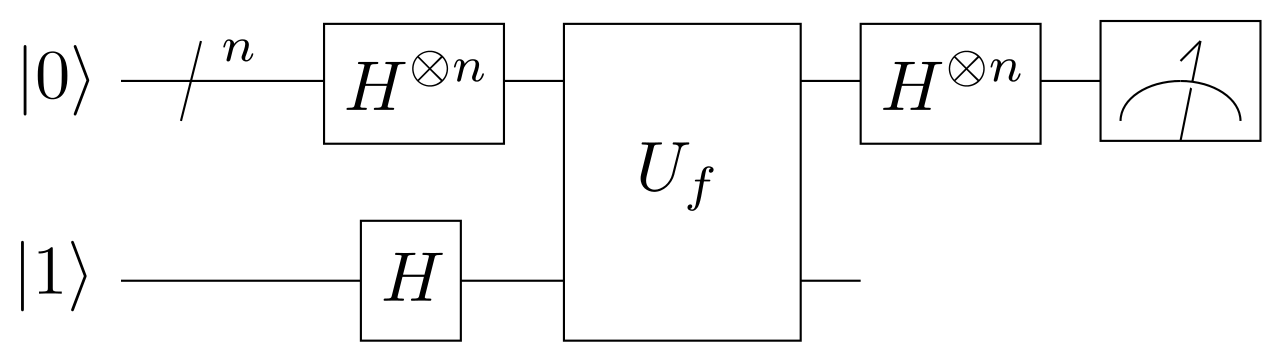
\includegraphics[scale=0.2]{Deutsch-Jozsa_Algorithm.png}
    \caption{Schéma de l'algorithme}
    \label{fig:univerise}
\end{figure}

\subsubsection{Initialisation}
On commence avec :
$\ket{u_0} = \ket{0}^{\bigotimes n}\ket{1}$
: n-qubits à $\ket{0}$ et 1-qubit à $\ket{1}$

\subsubsection{Etape 1}

On applique une porte de Hadamard à $\ket{u_0}$ pour avoir un état équiprobable:
$\ket{u_1} = H\ket{u_0} = \frac{1}{\sqrt{2^{n + 1}}}
\displaystyle\sum_{x=0}^{2^n-1} \ket{x}(\ket{0} - \ket{1})$

\subsubsection{Etape 2}
On applique l'oracle quantique suivant à $\ket{u_1}$: $\ket{x}\ket{y}\rightarrow\ket{x}\ket{y\oplus f(x)}$

Prenons le cas à 1 qubit:
\[
f(x) = 0: \ket{x}(\ket{0} - \ket{1}) \rightarrow \ket{x}(\ket{0} - \ket{1})
\]
\[
f(x) = 1: \ket{x}(\ket{0} - \ket{1}) \rightarrow \ket{x}(\ket{1} - \ket{0})
\]
\[
f(x) quelconque: \ket{x}(\ket{0} - \ket{1}) \rightarrow (-1)^{f(x)}\ket{x}(\ket{0} - \ket{1})
\]

En généralisant:

$\ket{u_2} = \frac{1}{\sqrt{2^{n + 1}}}
\displaystyle\sum_{x=0}^{2^n-1} (-1)^{f(x)}\ket{x}(\ket{0} - \ket{1})$

On peut ignorer le dernier qubit ($\ket{0} - \ket{1}$) comme il est
constant. Finalement, on en déduit :

$\ket{u_2} = \frac{1}{\sqrt{2^{n + 1}}}
\displaystyle\sum_{x=0}^{2^n-1} (-1)^{f(x)}\ket{x}$

\subsubsection{Etape 3}
On réapplique une porte Hadamard à chaque qubit sortant, ce qui donne:

$\ket{u_3} = \frac{1}{\sqrt{2^{n}}}
\displaystyle\sum_{x=0}^{2^n-1} (-1)^{f(x)} \displaystyle\sum_{y=0}^{2^n-1} (-1)^{x.y}\ket{y}$

$\ket{u_3} = \frac{1}{\sqrt{2^{n}}}
\displaystyle\sum_{x=0}^{2^n-1} \displaystyle\sum_{y=0}^{2^n-1}(-1)^{f(x)} (-1)^{x.y}\ket{y}$

La probabilité de mesurer $\ket{0}^{\bigotimes n}$ est : 
$|\frac{1}{\sqrt{2^{n}}}\displaystyle\sum_{x=0}^{2^n-1}(-1)^{f(x)}|$

Si on obtient 0, alors $f(x)$ est constante. Si on obtient 1, alors $f(x)$ est équilibrée.


\subsection{Example}

Prenons une fonction $f$ comme définie précédemment, sans savoir si elle est constante ou équilibrée.

\subsubsection{Etape 1}

On commence avec $\ket{u_0} = \ket{001}$. La première étape est l'application de la porte d'hadamard à $\ket{u_0}$: 
\medbreak
$
\ket{u_1} = H\ket{u_0} = H\ket{0} \otimes H\ket{0} \otimes H\ket{1}
$

$
\ket{u_1} = \frac{1}{2\sqrt{2}}\{ (\ket{0} + \ket{1})\otimes(\ket{0} + \ket{1})\otimes(\ket{0} - \ket{1}) \}
$

$
\ket{u_1} = \frac{1}{2\sqrt{2}}\{\ket{000} - \ket{001} + \ket{010} - \ket{011} + \ket{100} - \ket{101} + \ket{110} - \ket{111}\}
$

On peut factoriser le tout par $(\ket{0} - \ket{1})$: 

$
\ket{u_1} = \frac{1}{2\sqrt{2}}\{\ket{00}(\ket{0} - \ket{1}) + \ket{01}(\ket{0} - \ket{1}) + \ket{10}(\ket{0} - \ket{1}) + \ket{11}(\ket{0} - \ket{1})\}
$

\subsubsection{Etape 2: oracle quantique}

On applique à $\ket{u_1}$ l'oracle quantique $\ket{x}\ket{y}\rightarrow\ket{x}\ket{y\oplus f(x)}:$

$
\ket{u_2} = \frac{1}{2\sqrt{2}}[ \\ 
\ket{00}(\ket{0 \oplus f(00)} - \ket{1 \oplus f(00)}) + \\
\ket{01}(\ket{0 \oplus f(01)} - \ket{1 \oplus f(01)}) + \\
\ket{10}(\ket{0 \oplus f(10)} - \ket{1 \oplus f(10)}) + \\
\ket{11}(\ket{0 \oplus f(11)} - \ket{1 \oplus f(11)})]
$

\medbreak
On peut alors réécrire l'équation de la façon suivante: 

$
\ket{u_2} = \frac{1}{2\sqrt{2}}[ \\
(-1)^{f(00)} \ket{00}  (\ket{0} - \ket{1}) + \\
(-1)^{f(01)} \ket{01}  (\ket{0} - \ket{1}) + \\
(-1)^{f(10)} \ket{10}  (\ket{0} - \ket{1}) + \\
(-1)^{f(11)} \ket{11}  (\ket{0} - \ket{1}) ]
$

Par la suite, on va appliquer une porte de Hadamard à $\ket{u_2}$. Le qubit $\ket{0} - \ket{1}$ donne $\ket{1}$ par la cette porte, il est donc constant par rapport à $\ket{u_0}$. On peut donc le retirer de l'équation, ce qui nous donne pour $\ket{u_2}$ :
\medbreak
$
\ket{u_2} = \frac{1}{2\sqrt{2}}[(-1)^{f(00)} \ket{00} + (-1)^{f(01)} \ket{01} + (-1)^{f(10)} \ket{10} + (-1)^{f(11)} \ket{11} ]
$

\subsubsection{Etape 3: porte de Hadamard}

On applique donc une porte de hadamard à $\ket{u_2}$:

$
\ket{u_3} = \frac{1}{2\sqrt{2}} H [(-1)^{f(00)} \ket{00} + (-1)^{f(01)} \ket{01} + (-1)^{f(10)} \ket{10} + (-1)^{f(11)} \ket{11} ]
$

Nous sommes sur une porte de hadamard pour 2 qubits, ce qui donne l'équation matricielle suivante pour l'état $A$ de $\ket{u_3}$:

$
A=
\frac{1}{4\sqrt{2}} 
\begin{bmatrix}
  1 & 1 & 1 & 1 \\
  1 & -1 & 1 & -1 \\
  1 & 1 & -1 & -1 \\
  1 & -1 & -1 & 1 \\
\end{bmatrix}
\begin{bmatrix}
  (-1)^{f(00)} \\ (-1)^{f(01)} \\ (-1)^{f(10)} \\ (-1)^{f(11)}
\end{bmatrix}=
\frac{1}{4\sqrt{2}} 
\begin{bmatrix}
  (-1)^{f(00)} + (-1)^{f(01)} + (-1)^{f(10)} + (-1)^{f(11)} \\
  (-1)^{f(00)} - (-1)^{f(01)} + (-1)^{f(10)} - (-1)^{f(11)} \\
  (-1)^{f(00)} + (-1)^{f(01)} - (-1)^{f(10)} - (-1)^{f(11)} \\
  (-1)^{f(00)} - (-1)^{f(01)} - (-1)^{f(10)} + (-1)^{f(11)} \\
\end{bmatrix}
$
\medbreak
Si f est constante, alors $(-1)^{f(00)} = (-1)^{f(01)} = (-1)^{f(10)} = (-1)^{f(11)} = 1$. On a donc : 

$
A=
\frac{1}{\sqrt{2}} 
\begin{bmatrix}
  1 \\ 0 \\ 0 \\ 0
\end{bmatrix}
$

Et donc une probabilité de $1$ de mesurer l'état $\ket{00}$.

\medbreak
En revanche, si f est équilibrée, la moitié des valeurs vont valoir $(-1)^{0} = 1$ et l'autre moitié $(-1)^{1} = 0$. La première ligne du vecteur $A$ donne donc systématiquement 0, on ne mesure donc jamais l'état $\ket{00}$.

\medbreak

\end{document}
